%\chapter{USSS toolkits}
%shown in figure~\ref{fig:artificialnatural}
%pages~\pageref{tab:opposites1}
%and form (section~\ref{section:form}, page~\pageref{section:form}).

\chapter{Electronic Music 1}
\label{history1}

\section{The Early Days: The Futurists, The Dadaists, L`objet trouv\'e, Ives, Var\`ese, The RTF (Paris), WDR (Cologne) and the Studio di fonologia musicale Rai (Madrid)}

Where to start? Music, past and present? It does appear that electroacoustics (and by this term let's say anything involving electronics or computers) was trying to expand the palette of colour available to the composer. Many novel inventions (often in the guise of instruments) produced clear pitches that allowed them to be played in a classical manner but many more, produced new sounds of completely unknown origins. So much so that it has changed the way we perceive electronic sounds structured to form an artwork. Note I studiously avoid the word music! We might reflect that in this day and age you might well have an online (sonic) artwork in one window running in Flash whilst you finish your email! The whole conception and consumption of art is in a state of flux.

There are so many milestones in the development of electroacoustic music throughout the last 50 years that we will not be able to cover them all. However, whilst technology has developed in a very streamlined, linear, ever-onward fashion (only going retrograde by emulation or fashion), musical developments that have taken place are not so easily charted. In no way can one tie the sonic artworks of the time to any technology and we should not try to do so.

Grove Dictionary
\begin{itemize}
\item \href{http://www.grovemusic.com/shared/views/article.html?from=search&session_search_id=1011869954&session_name=e09647b5a66fbfeb&hitnum=1&section=music.08694&start=1&query=electronic%20instruments&search_subview=search_subject}{electronic instruments}
\item \href{http://www.grovemusic.com/shared/views/article.html?section=music.08695}{electroacoustic music}
\item \href{http://www.grovemusic.com/shared/views/article.html?section=music.40583}{computers and music}
\end{itemize}

\begin{itemize}
\item Changes in the way we listened to music - Var\`ese.
\item Futurists - Russolo
\item Thaddeus Cahill - Telharmonium
\item The Theremin - OHM Rockmore 

\end{itemize}

In August 1920 Leon Theremin (Lev Termen) - (b St Petersburg, 15 Aug 1896; d
Moscow, 3 Nov 1993) demonstrated the aetherphone later called the Theremin. In 1927
Theremin arrived in New York. His first appearance was a private demonstration concert
to guests including Joseph Szigeti, Arturo Toscanini and Sergei Rachmaninoff. Theremin
sold the licence for manufacture to the Radio Corporation of America (RCA).
Unfortunately, probably due to the technique required to make it sound ‘musical’, the
device never really took off.

However, some decided to conquer the theremin. The first virtuoso theremin player was
Clara Rockmore, a violinist who arrived from Russia in 1927. In 1938 Theremin was
abducted by Soviet agents and lived in Moscow for the majority his life.
\url{http://www.thereminworld.com/}

The theremin uses a ``beat frequency oscillator'' to combine the output from two radio
frequency oscillators, a process known as heterodyning. One oscillator operates at a fixed frequency,
which can be anything from 170,000 Hz to 282,000 Hz, depending on the theremin
model in question. The Ondes Martenot works in a similar fashion. [Maurice Martenot (b
Paris, 14 Oct 1898; d Clichy, nr Paris, 8 Oct 1980)]

\begin{figure}[H]
\centering
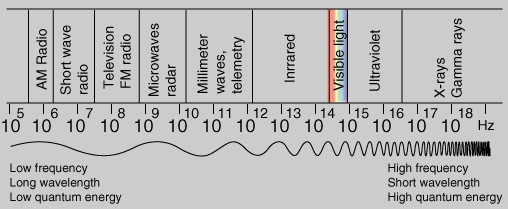
\includegraphics[scale=0.6]{waves}\caption{frequency scales}
\label{fig:waves to frequencies}
\end{figure}

\begin{itemize}
\item \href{http://www.grovemusic.com/shared/views/article.html?from=search&session_search_id=1013431856&session_name=f64e02b451f7a922&hitnum=1&section=music.00997&start=1&query=antheil&search_subview=search_subject}{Antheil} \textit{Ballet Mechanique} (1923-5)
\item \href{http://www.grovemusic.com/shared/views/article.html?from=search&session_search_id=1013432477&session_name=f64e02b451f7a922&hitnum=1&section=music.40105&start=1&query=satie&search_subview=search_subject}{Satie} \textit{Parade} (1917)
\item \href{http://www.grovemusic.com/shared/views/article.html?section=music.47335}{Respighi} \textit{Pines of Rome} (1924)
\item \href{http://www.grovemusic.com/shared/views/article.html?section=music.49908}{Cage} \textit{Imaginary Landscpes} (1939)
\item \href{http://www.grovemusic.com/shared/views/article.html?section=music.29042}{Var\`ese} \textit{Euqatorial} (1934), \textit{D\'eserts} (1950-54 ), \textit{Poem Electronique} (1958),
\end{itemize}


Futurists and Futurism:
\begin{itemize}
\item Filippo Tommaso Marinetti (1876-1944)
\item \href{http://www.grovemusic.com/shared/views/article.html?section=music.24174}{Luigi Russolo} (1885-1947)
\item \href{http://www.grovemusic.com/shared/views/article.html?from=search&session_search_id=1013432510&session_name=f64e02b451f7a922&hitnum=4&section=music.22259&start=1&query=marinetti&search_subview=search_subject}{Balilla Pratella} (1880-1965)
\end{itemize}

\begin{itemize}
\item Thaddeus Cahill (1867 - 1934) --- \href{http://www.grovemusic.com/shared/views/article.html?section=music.46183}{Telharmonium} 1897
\item \href{http://www.grovemusic.com/shared/views/article.html?section=music.45834}{Leon Theremin} (Lev Termen) (b St Petersburg, 15 Aug 1896; d Moscow, 3 Nov 1993)
\end{itemize}

\section{Pre-history 2}
\begin{itemize}
\item Electronic music developments in science and music
\item Schoenberg (1874-1951) - 5 orchestral pieces(1909) - III: Farben - Klangfarbenmelodie
\item Messiaen and the...Turanaglîla
\item Ondes Martenot - F\^te des Belles Eaux
\item Early Recording
\item Pierre Schaeffer in RTF - Cinq \'etudes de Bruits (1948) - \'Etudes aux objets (1959) - solfége
\item Jean Barraqu\'e - Etude (1953), Herbert Eimert + Robert Beyer - Klangstudie II (1952)
\item Stockhausen in RTF - Etude (1952)
\item Karlheinz Stockhausen in WDR - Electronishe Studies (1953, 1954), Gesang der J\"unglinge (1956), Kontakte (1960), Telemusik (1966), Hymnen (1966-7).
\end{itemize}

Schoenberg (writing to Mahler) ``..the possibility of creating a melody from one note played successively on different instruments''.

Messiaen (1908 - 1992): Oraison from 1937 is an extract from F\^ete des Belles Eaux. Commissioned and written for the world exposition in 1937

\begin{figure}[H]
\centering
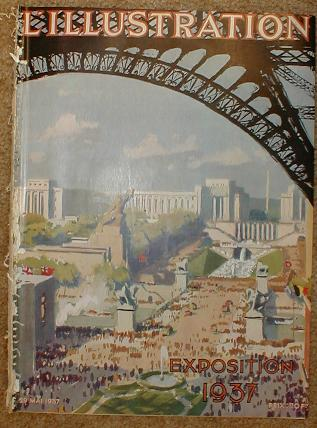
\includegraphics[scale=0.6]{illustration}\caption{world fair 1937}
\label{fig:worldfair}
\end{figure}

A Sons et lumi\'ere performance with fireworks and water jets. Twenty composers were commissioned. Many wrote orchestral works but Messiaen wrote for a sextet of Ondes Martenots. The music was amplified by loudspeakers placed buildings on the banks of the river Seine.

What does the ondes martenot do / look like?

\begin{figure}[H]
\centering
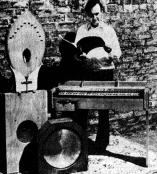
\includegraphics[scale=0.6]{mart}\caption{ondes martenot 1}
\label{fig:worldfair}
\end{figure}

\begin{figure}[H]
\centering
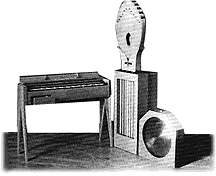
\includegraphics[scale=0.6]{martenot}\caption{ondes martenot 2}
\label{fig:worldfair}
\end{figure}

\subsection{Early Recording}
\begin{itemize}
\item Thomas Edison 1877, phonograph (hollow cylinder)
\item Emile Berliner 1887, flat disc gramophone
\item In 1925 Kurt Stille and partners licensed magnetic tape production to Ludwig Blattner and Kaul Bauer
\item In 1930 Marconi purchased Blattner's.
\item In Germany Fritz Pfleumer interested I.G.Farben in developing plastic backed tape (much lighter and safer) and Allgemeine Electrizitats Gesellsch\"ft (AEG) in developing machines. [by 1945 AEG had 15khz frequency response in magnetic tape at 30ips). Then the Minnesota Mining and Manufacture company developed a new tape (3M).
\end{itemize}

Sound in film - optical recordings had been around for some time and composers including the British composer Daphne Oram used this technique.

\section{Schaeffer (RTF) and Stockhausen (WDR)}

Schaeffer (1910-1995) and the GRM.

Studio d'Essai under German occupation 1942 / Club d'Essai in 1946. Groupe de Recherches Musicales (GRM) in 1958.

\begin{itemize}
\item Cinq \'etudes de Bruits (1948) - Concert de Bruits 1948
\item Symphonie pour un homme seul (1950) - with Pierre Henry (1927).
\item Etudes aux objets (1959)
\end{itemize}

\subsection{The Cologne studios}

Herbert Eimert (1897 - 1972), Robert Beyer (1901-1989) - Klangstudie II

\begin{enumerate}
\item demonstrate the analysis and synthesis of timbres:...
\item establish finely graduated scales between tone and noise
\item demonstrate the unity of musical time by creating graduated transitions between pitch and rhythm
\item use differentiated scales of loudness and reverberation to create a multi-layered spatial perspective.
\end{enumerate}

1948. Homer Dudley, from Bell Telephone Labs visited Werner Meyer Eppler.  Dudley had with him a new VOCODER – reactive filters on one side (reacting to sound A) that affect filters on the other side which filter Sound B. Robert Beyer was there from WDR. In 1950 they were joined by Herbert Eimert. Construction of the studio began in 1951/1952.  Bruno Maderna worked with Meyer-Eppler in Bonn (Institute of Phonetics, University of Bonn) and composed Musica su Due Dimensioni, (1952) for flute, percussion and tape which was performed that summer at Darmstadt to an audience that included PB, Gottfried Michael Koenig, Karel Goeyvaerts and KS.  The aesthetic was lead by Eimert who saw Elektronische Musik as an extension of serialism.

Serialism – understanding thereof.  Total serialism after Webern. 

KS began to work at WDR in May 1953.  \textit{Studie I} (1953) and \textit{Studie II} (1954) – see MUS201 / B+S course. Serial techniques to determine frequencies of sine waves.  Sounds being built up from first principles (Fourier after Helmholz).  Equipment resource consisted of a sine wave generator, a white noise generator, a melocord, and a monochord (a modified Trautonium built by Trautwein).  Most people (including KS) preferred to use the sine wave generator and a multitrack tape recorder.

\textit{Gesang der J\"unglinge} (1956) – mixture of natural and electronic but not a piece of musique concr\`ete by any means. (See B+S course).  A step away from serialism too with the warmth of natural colours and the pointillistic clouds.

1960 Stockhausen completed Kontakte.  Solo tape and tape + percussion + piano.  Moment Form.
 
During a visit to Japan he composed Telemusik (tele – all) – ring modulation.  1965, Solo for melody instrument with feeback.  1967 saw the completion of Hymnen.  Much intermodulation, ring modulation by high frequencies or rich modulation freqs that truly fused two signals – result often not an audible sign of either hence the mystical tag.  Stockhausen rubbished musique concr\`ete even then as `primitive collage'. 

He was director of WDR from 1962 to 1980.  Impressive list of equipment.  Composers attending during that time:

Gottfried Michael Koenig, Gyögy Ligeti, Mauricio Kagel, Konrad Boehmer, Mesias Maiguashca, Bernd Alois Zimmermann, York H\"oller, Roger Smalley, Jean-Claude Eloy, Tim Souster, Luc Ferrari, Iannis Xenakis.

\subsection{Var\`ese}
\begin{itemize}
\item 1920-21		Am\'eriques
\item 1921		Offrandes
\item 1922-23		Hyperprism
\item 1923		Octandre
\item 1923-25		Int\'egrales
\item 1926-27		Arcana
\item 1931		Ionisation
\item 1934		Ecuatorial
\item 1936		Density 21.5
\item 1950-54		D\'eserts
\item 1958		le Poem \'electronique
\item 1961		Nocturnal
\item 1965		Night (unfinished)
\end{itemize}

1916 Varèse said – ``Our musical alphabet must be enriched...we also need new instruments badly''.  The continuous flowing curve generated by the siren – (manual version of the oscillator). Var\`ese's ideas for an instrument similar to the Theremin was the Dynaphone.  Applications were made to the Guggenheim Foundation but were not successful. 

1954 – Var\`ese in Paris for tape parts for D\`eserts. 1957 – Philips Labs in Eindhoven, Holland for Poème Electronique.  There he met Xenakis. World's Fair in May 1958: Le Corbusier, (Charles-Edouard Jeanneret) (Le Corbusier) b1887 – 1965. Var\`ese and Xenakis. Music on a 3 track tape distributed over 425 loudspeakers.

\begin{itemize}
\item 1952 Konkrete Et\"ude (concrete music) - Stockhausen working with Schaeffer and studying with Messiaen
\item 1953 Elektronische Studie I
\item 1954 Electronische Studie II
\item 1955-6 Gesang der J\"nglinge
\item 1959-60 Kontakte (electronic and version for piano, percussion and electronics)
\item 1966 Telemusic (electronic music)
\item 1966 Hymnen (electronic and concrete music) - version with soloists - 1969 version with orchestra
\end{itemize}

\subsection{Japan}
1951 also in Japan: Tokyo
Joji Yuasa, Toru Takemistsu, Hiroyoshi Suzuki, Kazuo Fukushima founded Jikken Kobo (an experimental workshop). 1953 at NHK (Nippon Houso Kyokai / Japanese Broadcasting Corporation).  Joji Yuasa is perhaps best known out of the NHK crowd.

